\section{Results and Discussion}
%For example, if the distance of one point is larger than three sigmas, 
%we treat this point as an outlier in Algorithm~\ref{alg:kmeans}.
All three methods were applied to five meteorological variables across
all facilities. The methods identified different sets of outlier events,
with some events identified by more than one methods
(Figures~\ref{fig:pc},\ref{fig:ssa},\ref{fig:kmeans}).
% methods drawbacks and advantages

Among three methods Pearson correlation was least effective with
frequent false negatives.
That is due to the fact that pairwise Pearson correlation method was 
applied at seasonal scale, thus was only able to find large outliers.
Pearson correlation coefficient is a pairwise comparison method, however, 
if the two variables deviates in the same direction, their correlation 
may not change significantly and thus may go undetected. Due to seasonal
nature of the analysis, it was not able to identify ouliers that
persisted at hours to days only.
Univariate SSA method was very effective at identifying outlier high and
low values in the time series with high \textit{Precision} but low \textit{Recall}. 
$k$-means based outlier detection was also able to identify outliers
with high \textit{Precision} and low \textit{Recall}. 



\begin{table}[ht]
\caption{Comparison of SSA and K-means Outlier Set Size}
\label{tab:comp}
\centering
\begin{tabular}{|l|c|}
\cline{2-2}
\multicolumn{1}{l|}{} & Outlier Set Size\\
\hline
SSA & 922\\
K-means & 508\\
Intersection & 378\\
Symmetric Difference & 674\\
\hline
\end{tabular}
\end{table}

\begin{table}[ht]
\caption{Precision and Recall of SSA and K-means}
\label{tab:pr}
\centering
\begin{tabular}{|l|c|c|c|}
\hline
Method & Variable & Precision & Recall\\
\hline
SSA & temp\_mean & 16.00\% & 1.20\%\\
SSA & vapor\_pressure\_mean & 20.70\% & 1.40\%\\
SSA & atmos\_pressure & 0.00\% & 0.00\%\\
SSA & rh\_mean & 14.80\% & 0.50\%\\
SSA & wspd\_arith\_mean & 0.60\% & 1.50\%\\
Kmeans & 5 together & 12.90\% & 1.90\%\\
Combined & 5 together & 11.10\% & 4.10\%\\
\hline
\end{tabular}
\end{table}

%K-means is a commonly used multivariate method 
%for clustering. Here we used it for outlier detection. The drawback of this method is 
%that the detected outliers could be just one type of variable or 
%multiple types of variable. It is hard to tell which is the case for 
%correcting the new data. As we also averaged the raw 
%minute level data into day level data, some outliers may be averaged 
%out by this process.

% all together as a template
SSA method identified largest number of outlier events (922)
(Table~\ref{tab:comp}) across the entire dataset, while $k$-means
identified 508 events. While 378 events were identified as outlier by
both the methods (intersection), 674 events were only identified by one
of the methods (Table~\ref{tab:comp}).
Figure~\ref{fig:combined} show all the outliers detected by SSA and
$k$-means methods at facility E33 for \textit{temp\_mean}. 
When combined together developed outlier detection methods had
\textit{Precision} of 11.10\% which show that many of the outliers
detected are not within ARM DQR database, which is a know limitation of
the current records that this current study is trying to address.
Detected outliers also had low \textit{Recall} which in addition to small
number of true positives can be due to fact that DQR database often
record a wide affected date range for an identified outlier instead of a
precise date thus leading to large false negatives, all of which leads
to low \textit{Recall} values.

Overall, when combined together within a framework, set of methods applied allows
to capture outlier events caused by a wide range of conditions. 

%One outlier may only be detected by SSA or Pearson correlation coefficient 
%or K-means. Thus we combined all the three methods together as a 
%whole framework. SSA and K-means are used to detect outliers whereas Pearson 
%correlation coefficient can be used to detect the variables causing the anomaly 
%in the K-means results by using the pairwise correlations. Figure~\ref{fig:combined} is the result of 
%detected outliers for \textit{temp\_mean} from E33. 
%The red squares 
%stand for the common outliers detected by both K-means and SSA. The 
%orange diamonds are the ones detected by K-means excluding the common 
%outliers. And the black stars represents the outliers detected by SSA 
%excluding the common outliers. We can see from the figure that more 
%outliers have been detected compared to Figure~\ref{fig:ssa} and Figure~\ref{fig:kmeans}. 
%Thus we applied this framework on all the test data. Table~\ref{tab:comp} 
%shows the number of detected outliers. The size of common detected 
%outliers is 378 by this framework.

\begin{figure*}[ht]
    \centering
    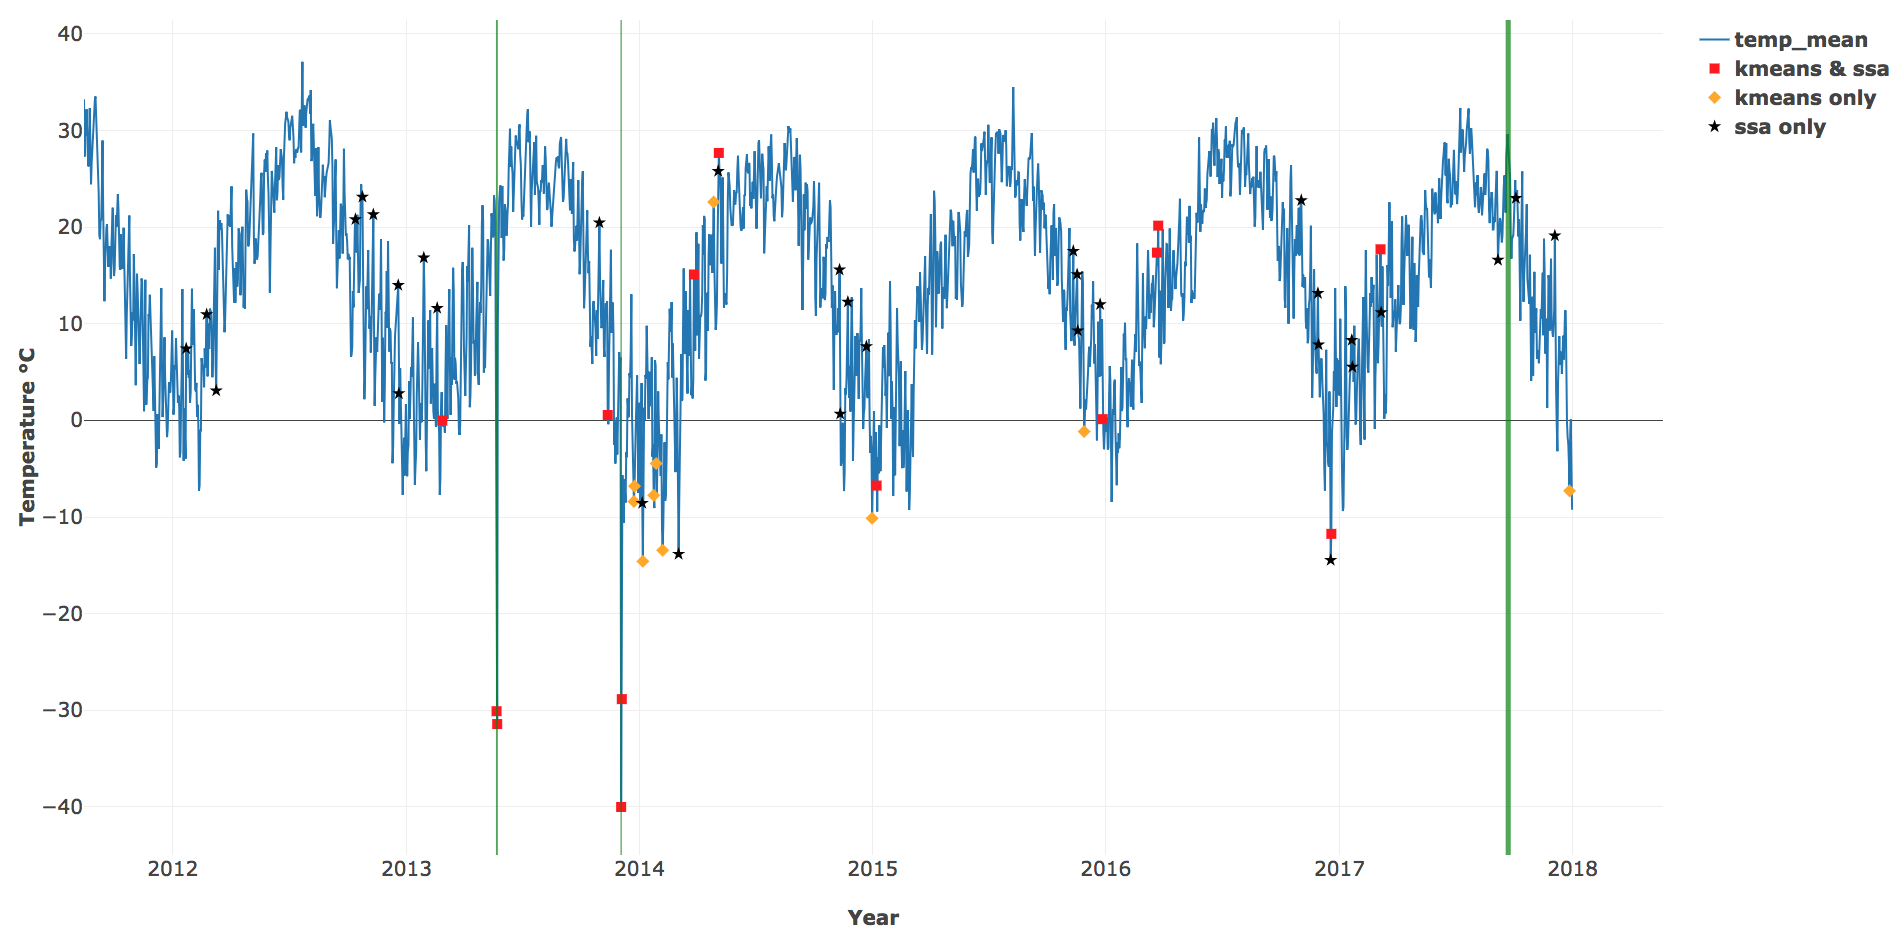
\includegraphics[width=\textwidth]{figures/combined.png}
    \caption{Outliers detected at facility E33 for \textit{temp\_mean}
		by SSA and $k$-means algorithms. Outliers detected by both
		algorithms are shown by red squares, while those identifed by
		SSA and $k$-means only are indicated by black stars and orange
		diamonds respectively. DQR records are denoted by the green shaded areas.}
    \label{fig:combined}
\end{figure*}

% DQR here
%The current data quality or outlier detection is maintained as data 
%quality reports (DQRs) stored in the DQR database with each entered 
%manually \cite{mccord2016arm}. A description of an event which 
%changed the normal data is included in these DQRs. The event could 
%be temporary operating conditions such as power failures, frozen 
%and snow covered sensors, instrument degradation, or contamination. 
%It could also be an extreme weather event that has never been observed 
%before. Each DQR entry also contains a specific time range affected, 
%list of data projects, and specific measurements. And these entries 
%are usually submitted by either the Data Quality Office \cite{peppler2016arm} 
%or the instrument mentor \cite{cress2016deploying}. It is easy to 
%notice that this method is not efficient as it requires a lot of labor. 
%It is also nearly impossible to detect all the outliers due to the 
%complexity and high volume of the ARM data.

%Currently, not many outliers entries are stored in DQR database. Here we 
%used manually detected 181 outliers in the DQR database as the ground 
%truth to compare with the results from our framework. Precision and 
%recall which were first defined in \cite{perry1955machine} were used 
%as the comparison metric. They are commonly used to measure the quality 
%of classification tasks \cite{olson2008advanced}. Precision is calculated 
%as True Positives divided by the sum of True Positives and False 
%Positives. On the other hand, recall is measured from True Positives 
%divided by the sum of True Positives and False Negatives. We treated 
%outliers in DQR database as True Positives. Thus detected outliers not 
%in the DQR database are False Positives. Undetected values which in 
%the DQR database are False Negatives, and which not in the DQR database 
%are True Negatives. Table~\ref{tab:pr} contains the statistics of 
%the comparison.
%
%Precision attempts to answer the proportion of positive identifications that
%was actually correct. The Combined precision is 11.10\% which shows that 
%many outliers detected by the framework are not in the DQR database. 
%Recall tries to solve the proportion of actual positives identified 
%correctly. The number is 4.10\% which is even smaller than precision. 
%One reason for small recall is that the size of True Positives 
%is much small. The other reason is that DQR database records the whole 
%possible affected time range which makes the size of False Negatives 
%large. It could be possible that only a few days of the data recorded 
%during that time range are actually outliers.

